\lstset{style=customcpp}
The firmware developed for the ESP32 is the core of the Mecanum wheel car's control system, responsible for managing communication protocols, motor control, and system monitoring. The structure of the firmware has been designed to handle different modes of operation, including control via WiFi and Bluetooth, while providing real-time feedback on the car’s status, including battery level monitoring.\\
The firmware begins with the inclusion of essential libraries such as MotorPWM, UDPcontrol, PS4Control, BatteryStatus, and StatusLED. These libraries are integral to the car's operation, providing control over motor speed via PWM, handling the UDP or PS4 control modes, monitoring battery levels, and updating LED indicators for status feedback.\\
The user can choose between two control modes by defining either \lstinline|UDP_CONTROL_MODE| or \lstinline|PS4_CONTROL_MODE|. Only one of these modes should be active at any time, controlling whether the car is operated via WiFi (\acs{udp}) or through a PS4 controller using Bluetooth.
The \lstinline|SERIAL_DEBUG| define can be uncommented to enable serial debugging, which prints relevant system information such as motor speeds and battery levels to the serial monitor. This is useful for development and testing.\\

The \lstinline|setup()| function is responsible for initializing all key components, including the status LED, playing the startup animation indicating successful booting, and to start the communication processes. At the end of the startup process the battery value is checked once to store it in memory. Additionally memory space is reserved for the motor control arrays where the control input from the user is and the \ac{pwm} values for motors are stored. The whole process can be seen in fig.~\ref{fig:SetuopSequence}.

\begin{figure}[h]
	\centering
	\captionsetup{justification=centering}
	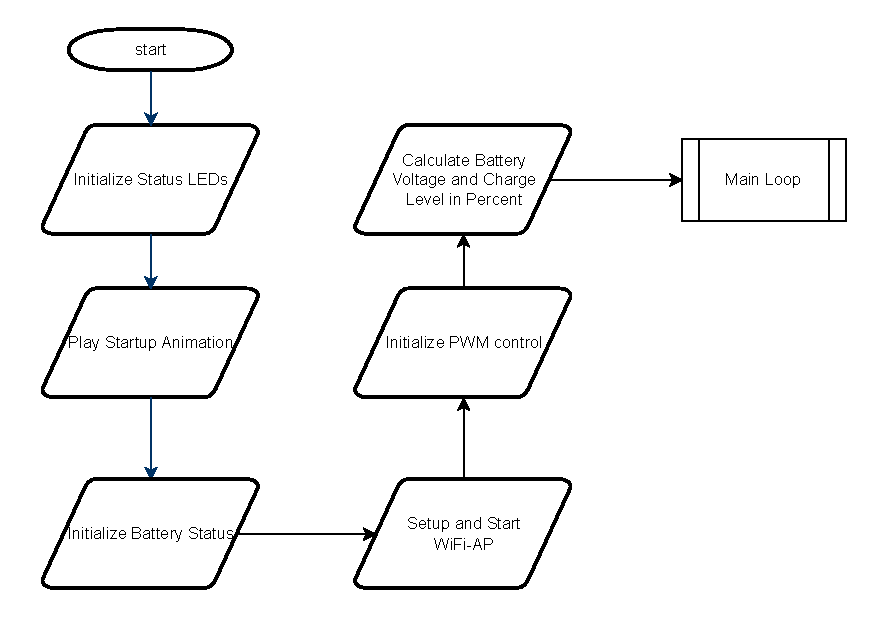
\includegraphics[width=1\linewidth]{Boot_Sequence_WiFiAP.pdf}
	\caption{Setup Sequence of Microprocessor}
	\label{fig:SetuopSequence}
\end{figure}

Afterwards the main \lstinline|loop()| function is entered, which loops infinitely. This function continuously checks for control input by the user and updates the motor outputs. 

 This function is the main execution loop that continuously checks for control input (either from UDP packets or PS4 controller), calculates motor speeds, and updates the motor outputs. It also checks the battery status every second and sends status messages back to the controller in UDP mode. At the same time this function checks the battery status periodically and sends the status message back to the user after a specified time interval passes. This process can be seen in fig.~\ref{fig:MainLoopSequence}.

\begin{figure}[h]
	\centering
	\captionsetup{justification=centering}
	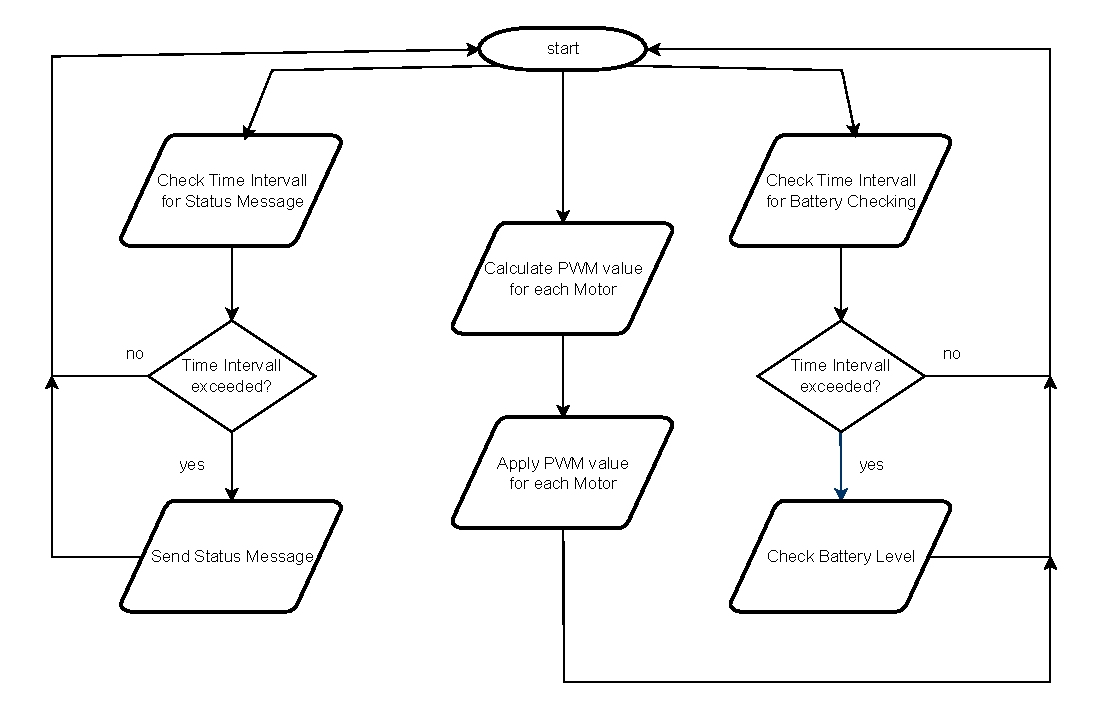
\includegraphics[width=1\linewidth]{LoopSequence_WiFiAP.pdf}
	\caption{Main Loop Sequence of Microprocessor}
	\label{fig:MainLoopSequence}
\end{figure}

The firmware for the ESP32 microcontroller plays a crucial role in the operation of the Mecanum wheel car. It efficiently manages the control modes, motor control, and system monitoring while providing flexibility in terms of communication protocols (WiFi/UDP or Bluetooth). The modularity of the firmware allows for future extensions and adjustments as needed for enhanced functionality or new features. For example new sensors can be added which are checked at the same time as the battery level. The status message can also be expanded to accustom for more sensor data that needs to be transmitted.